
\let\negmedspace\undefined
\let\negthickspace\undefined
\documentclass[journal]{IEEEtran}
\usepackage[a5paper, margin=10mm, onecolumn]{geometry}
%\usepackage{lmodern} % Ensure lmodern is loaded for pdflatex
\usepackage{tfrupee} % Include tfrupee package
\setlength{\headheight}{1cm} % Set the height of the header box
\setlength{\headsep}{0mm}     % Set the distance between the header box and the top of the text
\usepackage{gvv-book}
\usepackage{gvv}
\usepackage{cite}
\usepackage{amsmath,amssymb,amsfonts,amsthm}
\usepackage{algorithmic}
\usepackage{graphicx}
\usepackage{textcomp}
\usepackage{xcolor}
\usepackage{txfonts}
\usepackage{listings}
\usepackage{enumitem}
\usepackage{mathtools}
\usepackage{gensymb}
\usepackage{comment}
\usepackage[breaklinks=true]{hyperref}
\usepackage{tkz-euclide} 
\usepackage{listings}
% \usepackage{gvv}                                        
\def\inputGnumericTable{}                                 
\usepackage[latin1]{inputenc}                                
\usepackage{color}                                            
\usepackage{array}                                            
\usepackage{longtable}                                       
\usepackage{calc}                                             
\usepackage{multirow}                                         
\usepackage{hhline}                                           
\usepackage{ifthen}                                           
\usepackage{lscape}
\renewcommand{\thefigure}{\theenumi}
\renewcommand{\thetable}{\theenumi}
\setlength{\intextsep}{10pt} % Space between text and floats
\numberwithin{equation}{enumi}
\numberwithin{figure}{enumi}
\renewcommand{\thetable}{\theenumi}
\begin{document}
\bibliographystyle{IEEEtran}
\title{Question 7-7.2-18}
\author{EE24BTECH11041 - Mohit}
% \maketitle
% \newpage
% \bigskip
{\let\newpage\relax\maketitle}
\begin{enumerate}
	\item Equation of the circle with centre on the $Y$ axis and passing through the orgin and the point (2, 3) is
\begin{enumerate}
\item $x^2+y^2+6x+6y+3=0$ 
\item $x^2+y^2-6x-6y-9=0$
\item $x^2+y^2-6x-6y+9=0$
\item none of these
\end{enumerate}
\end{enumerate}
\begin{table}[h!]    
  \centering
  \begin{tabular}[12pt]{ |c| c|}
    \hline
    \textbf{Variable} & \textbf{Description} \\ 
    \hline
    $\vec{x_1}$ & Point on circle \\
    \hline
    $\vec{x_2}$ & Point on circle \\
    \hline 
    $\vec{n}$ &  Equation of line on centre of circle lies \\
    \hline   
    \end{tabular}

  \caption{Variables Used}
  \label{tab 1.4.9.2}
\end{table}
Solution:-\\
\begin{align}
	\vec{x}_{1} = \myvec{2\\3},\ \vec{x}_{2} = \myvec{0\\0},\
	\vec{n} = \myvec{1 \\ 0},\  c= 0.
\end{align}
The centre is given by
\begin{align}
\myvec{
 2 \vec{x}_1 & 2 \vec{x}_2 & \vec{n}
 \\
 1 & 1 & 0
 }^\top 
	\myvec{\vec{u} \\ f}
	=
-\myvec{ 	\norm{\vec{x}_1}^2 
\\
 	\norm{\vec{x}_2}^2 	
	\\
	c     
	}
\end{align}
Substituting values of $\vec{x}_1$,$\vec{x}_2$ and $n$
\begin{align}
	\myvec{
	        4 & 6 & 1\\
	        0 & 0 & 1\\
-1 & 0 & 0}
	\myvec{\vec{u}\\f} = 
	\myvec{-13 \\ 0 \\ 0}
\end{align}
The augmented matrix is expressed as
\begin{align}
	\myvec{
	        4 & 6 & 1 & \vrule & -13\\
	       0 & 0 & 1 & \vrule & 0\\
-1 & 0 & 0 & \vrule & 0}
\end{align}
Performing a sequence of row operations to transform into an Echelon form
\begin{align*}
	\xleftrightarrow[]{{R_1\leftrightarrow R_3}}
	\myvec{1 & 0 & 0 & \vrule & 0\\
	        0 &  0 & 1 & \vrule & 0\\
	        4 & 6 & 1 & \vrule & -13}
	\xleftrightarrow[]{{R_3\rightarrow R_3-4R_1}}
	\myvec{1 & 0 & 0 & \vrule & 0\\
	        0 &  0 & 1 & \vrule & 0\\
	        0 &  6 & 1 & \vrule & -13}\\
	\xleftrightarrow[]{{}}
	\myvec{ 1 & 0 & 0 & \vrule & 0\\
	        0 &  1 & \frac{1}{6} & \vrule & -\frac{13}{6}\\
	        0 &  0 & 1 & \vrule & 0}	
	\xleftrightarrow[]{{R_2\rightarrow R_2-\frac{1}{6}R_3}}
	\myvec{ 1 &  0 & 0 & \vrule & 0\\
	        0 &  1 & 0 & \vrule & -\frac{13}{6}\\
	        0 &  0 & 1 & \vrule & 0}
\end{align*}
So,the values of $\vec{u}$ and $f$ are
\begin{align}
	\vec{u} = -\myvec{0\\\frac{13}{6}},\
	f = 0.
\end{align}
The radius of circle is
\begin{align}
	r=\sqrt{(\norm{\vec{u}}^2-f)}=\frac{13}{6}
\end{align}
The equation of circle is
\begin{align}
	\norm{\vec{x}}^2-2\myvec{0 & \frac{13}{6}}\vec{x}=0
\end{align}
OR
\begin{align}
x^2+y^2-\frac{13}{3}y=0
\end{align}
Hence,option (d) is correct
\begin{figure}[h!]
   \centering
   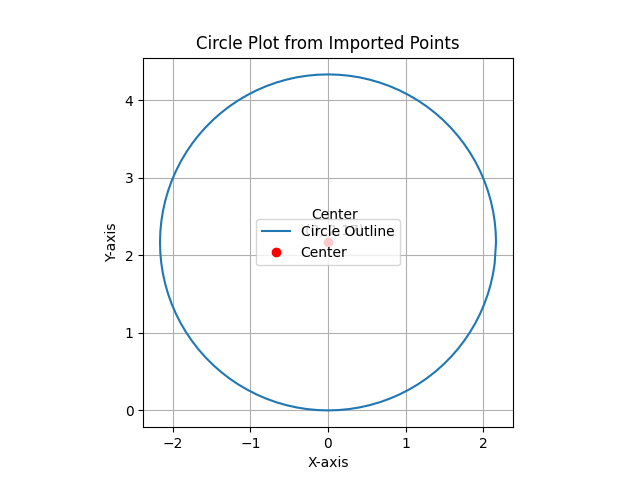
\includegraphics[width=0.7\linewidth]{figs/Figure_1.png}
   \caption{Plot of circle}
   \label{stemplot}
\end{figure}
\end{document}
